\documentclass[12pt]{article}

\usepackage{wrapfig}
\usepackage{float}
\usepackage{graphicx}
\usepackage[margin=1in]{geometry} 
\usepackage{comment}
\usepackage{amsmath,amsthm,amssymb}
\usepackage{hyperref}
% \usepackage[vlined,linesnumbered,ruled,resetcount]{algorithm2e}
\usepackage{algorithm}
\usepackage[noend]{algpseudocode}
\usepackage{tikz}

% the following nonsense allows you to put a comment below a big algorithm
\usepackage{etoolbox}
\makeatletter
\AfterEndEnvironment{algorithm}{\let\@algcomment\relax}
\AtEndEnvironment{algorithm}{\kern2pt\hrule\relax\vskip3pt\@algcomment}
\let\@algcomment\relax
\newcommand\algcomment[1]{\def\@algcomment{#1}}

\renewcommand\fs@ruled{\def\@fs@cfont{\bfseries}\let\@fs@capt\floatc@ruled
  \def\@fs@pre{\hrule height.8pt depth0pt \kern2pt}%
  \def\@fs@post{}%
  \def\@fs@mid{\kern2pt\hrule\kern2pt}%
  \let\@fs@iftopcapt\iftrue}
\makeatother


\DeclareMathOperator*{\argmax}{arg\,max}
\DeclareMathOperator*{\argmin}{arg\,min}
\DeclareMathOperator*{\val}{val}
\DeclareMathOperator*{\MOSM}{MOSM}
\DeclareMathOperator*{\WOSM}{WOSM}
\DeclareMathOperator*{\best}{best}
\DeclareMathOperator*{\worst}{worst}

\newcommand{\R}{\mathbb{R}}
\newcommand{\Rgz}{\mathbb{R}_{\ge 0}}
\newcommand{\N}{\mathbb{N}}
\newcommand{\Z}{\mathbb{Z}}

\newcommand{\Es}[2]{\mathbb{E}_{#1}\left[{#2}\right]}
\newcommand{\E}[1]{\mathbb{E}\left[{#1}\right]}
\newcommand{\ip}[2]{\left\langle{#1} , {#2}\right\rangle}

\newcommand{\M}{\mathcal{M}}
\newcommand{\W}{\mathcal{W}}
\renewcommand{\L}{\mathcal{L}}

\newtheorem{definition}{Definition}[section]
\newtheorem{lemma}[definition]{Lemma}
\newtheorem{corollary}[definition]{Corollary}
\newtheorem{theorem}[definition]{Theorem}
\newtheorem{claim}[definition]{Claim}
\newtheorem{proposition}[definition]{Proposition}

\begin{document}

% \renewcommand{\qedsymbol}{\filledbox}
 
\title{
  Efficiently Representing the Set of Stable Matchings by the Rotation Poset
}
\author{
  Clay Thomas\\
  claytont@princeton.edu
}
\maketitle

\begin{abstract}
  Stable matchings are a classical area of study, and
  the well-known treatment of [Gusfield and Irving. ``The stable
    marriage problem: structure and algorithms". MIT press, 1989]
  gives strong structural results useful for understanding this problem.
  Namely, the set of stable matchings for an $n\times n$
  instance is in a bijection with the set of downward-closed subsets of a
  certain polynomial-sized partial order (the elements of which correspond to
  the set of stability-preserving ``partner rotations'').
  While Gusfield and Irving's treatment is quite elegant,
  the proofs given are a bit long and abstract.
  In this paper, we give a slight modification of
  the Gusfield and Irving algorithm, emphasizing its conceptual basis
  in the same principles as differed acceptance.
  We prove correctness mostly by using concrete algorithmic properties.
  We also provide a more streamlined and
  unified construction of the partial ordering relations, correcting some
  slight errors in the original text.
  Our algorithm naturally handles unacceptable pairs
  and unequal numbers of men and women.

  We also discuss two recent advancements in the theory of \emph{counting}
  stable matchings. First, using basic properties of the partial
  order on rotations (which we reprove), a exponential worst-case upper bound on the
  number of stable matchings has been shown in 
  [Karlin, Gharan, and Weber. ``A simply exponential upper bound on the maximum
    number of stable matchings." STOC, 2018].
  Second, upper bounds for the \emph{expected}
  number of stable matchings when there are an unequal number of men and women
  have recently been found in [Ashlagi, Kanoria, and Leshno.
    ``Unbalanced random matching markets: The stark effect of competition."
    Journal of Political Economy, 2017]
  (it turns out there are far fewer matches than in the balanced case).
  For the second result, we provide greatly simplified proofs of some
  preliminary results in this direction.
\end{abstract}

\section{Introduction}

  Stable matching mechanisms are ubiquitous in theory and in practice,
  especially in the ``bipartite case'' where agents lie in two disjoint groups
  and matches are made between members of different groups.
  % Stable matchings present one of the rare examples in mechanism design without
  % money where many positive results are possible.
  The most commonly used stable matching mechanism is ``one-side proposing
  differed acceptance'', which has the nice properties of being simple to
  implement, fast to execute, and strategyproof for the proposing side
  \cite{DubinsMachiavelliGaleShapley81}
  (moreover, it is the unique mechanism satisfying strategyproofness for 
  one of the sides \cite{GaleMsMachiavelli85}).

  Many structural properties are known about the set of stable matches for a
  given instance (known as the \emph{core} of the instance).
  For instance, the core forms a distributive lattice with a compact
  (and algorithmically friendly) representation,
  and every distributive lattice is the core of some ``not too large''
  stable marriage instance \cite{IrvingCountingStable86}.
  This latter fact means that, a priori, one cannot say much more
  about the core than one can say about arbitrary distributive
  lattices\footnote{
    One recent result which runs counter to this statement is given in
    \cite{KarlinExpUBNumberStable18}, where the authors use the 
    size of the stable marriage instance to
    bound the number of elements in the distributive lattice of the core.
    There, the exact meaning of the words ``not too large'' becomes important.
  }. However, in addition to the structure that the core must necessarily have,
  it is very interesting to know what qualities the core \emph{probably} has.

  The ``first'' randomized model of stable matching is to take preferences
  completely uniform for each agent.
  For a while, it's been known that in a randomized balanced market,
  i.e. one with the same
  number of agents on each side, there's probably a large core
  and a big imbalance between the different sides -- the proposing side gets
  matched which they favor significantly more \cite{PittelAverageStable89}.
  However, in a recent breakthrough paper \cite{AshlagiUnbalancedCompetition17},
  it was found that this distinction
  \emph{almost vanishes} in large markets when there is an imbalance of just
  \emph{one} more agents on one side than the other.
  In this note we survey this result.

  The basic setup of stable matching has many variations.
  The central focus of this note is the setting with an unequal number of agents
  on each side.
  Some other import variations include adding ``unacceptable matches'' (agents do not
  rank every agent on the other side), ``indifference'' (agents sometimes don't
  distinguish their preference between some matches), ``many-to-one matchings''
  (where several agents from one side are matched to one on the other),
  and ``couples'' (where certain agents on one side express their 
  preferences/acceptable matches jointly).
  We use the ``unacceptable matches'' concept as a technical tool,
  but ignore the subtleties of the other variations.

  \paragraph{Relation to prior work.}
  No claim in this paper is original, and much of our treatment and proofs are
  very similar to that presented in \cite{GusfieldStableStructureAlgs89}.
  The point where we start to differ is in proving results about the rotation
  poset: we use the concepts of women truncating their preference lists and
  running MPDA to prove most of our claims.
  This approach has been surveyed in \cite{ManloveMatchPrefs13}.

  ==== HERM actually idk things were pretty clear to begin with in all these
  proof... but whatever. I'm still not sure how different my algorithm is from
  anything else.

  \paragraph{Organization.}
  In section 2, we review the basic properties of differed acceptance and stable
  matchings, which will motivate some of the techniques to come.
  In section 3, we review the case of a balanced market, and discuss which parts
  of the analysis fail for unbalance markets.
  In section 4, we prove some results on unbalanced markets, taking a new proof
  approach based around differed acceptance which is closer to the analysis for
  the balanced market.
  In section 5, we discuss the proof technique given in
  \cite{AshlagiUnbalancedCompetition17}.
  % and describe its relationship to algorithms previously known about the
  % structure of the core (from \cite{GusfieldStableStructureAlgs89}).

\section{Review: Differed Acceptance and Stable Matching}


  We start with the basic definitions.
  A matching market is a collection $\M$ of ``men'' and $\W$ of ``women'', where
  each man $m\in \M$ has a ranking over women in $\W$, represented
  as list ordered from most preferred to least preferred, and vice versa.
  Lists may be partial, and agents included on the list of some $a \in \M\cup\W$
  are called the acceptable partners of $a$.
  We write $w_1 \succ_m w_2$ if $w_1$ is ranked higher than $w_2$ on $m$'s list
  (or if $w_1$ is acceptable but $w_2$ is not ranked at all).
  We also denote the fact that $w$ is not an acceptable partner of $m$ by
  $\emptyset \succ_m w$.

  === More defining to do here::
  A matching is a one-to-one assignment of men to women, which we denote
  by $\mu : \M\cup \W\to \M\cup \W\cup\{\emptyset\}$.
  We write $\mu(i) = \emptyset$ if
  agent $i$ is unmatched.

  A matching $\mu$ is \emph{stable} for a set of preferences 
  $P = \{\succ_w\}_{w\in\W} \cup \{\succ_m\}_{m\in\M}$
  if no unmatched man/woman pair 
  $(m,w)\in \M\times \W$ is blocking under $P$,
  % we do not simultaneously have
  % $m \succ_w \mu(w)$ and $w \succ_m \mu(w)$.
  where $(m,w)$ is called blocking if we simultaneously have
  $m \succ_w \mu(w)$ and $w \succ_m \mu(w)$.
  A \emph{pair} $(m,w)$ is called stable under $P$ if $\mu(m)=w$ in 
  \emph{some} stable matching,
  and $m$ is called a stable partner of $w$ (and vice-versa).

  The man-proposing differed acceptance algorithm is given by
  Algorithm~\ref{algoMPDA}. We provide simple proof of the basic properties of
  this algorithm.

  \begin{algorithm}
    \caption{MPDA: Men-proposing differed acceptance algorithm}
    \label{algoMPDA}
  \begin{algorithmic}[0]
    \State Let $U = \M$ be the set of unmatched men
    \State Let $\mu$ be an all empty matching
    \While { $U\ne \emptyset$ and some $m\in U$ has not proposed to every woman
      on his list}
      \State Pick such a $m$ (in any order)
      \State $m$ ``proposes'' to their highest-ranked woman $w$ which 
        they have not yet proposed to
      \If {$m \succ_w \mu(w)$} 
        \State If $\mu(w)\ne \emptyset$, add $\mu(w)$ to $U$
        \State Set $\mu(w) = m$, remove $m$ from $U$ 
      % \EndIf
      % \If {$\mu(h) = d_0$ and $d\succ_h d_0$} 
      %   \State Set $\mu(h) = d$, remove $d$ from $U$, add $d_0$ to $U$
      % \Else \ \ $h$ remains matched to $d_0$ and $d$ remains in $U$
      \EndIf
    \EndWhile
  \end{algorithmic}
  \end{algorithm}

  Intuitively, this algorithm starts with the men doing whatever they prefer
  the most, then doing the minimal amount of work to make the matching stable.
  Indeed, men propose in their order of preference. If a woman $w$ ever
  rejected a man $m$ they prefer over their current match,
  then \emph{remained} with their current match,
  then $(m,w)$ would clearly create an instability in the final matching.

  \begin{claim}
    The output of MPDA is a stable matching.
  \end{claim}
  \begin{proof}
    First, observe that the MPDA algorithm terminates
    because every man will propose to every woman at most once.
    The claim follows from two simple invariants of the algorithm:
    \begin{itemize}
      \item Men propose in their order of preference
      \item Women can only increase the rank of their tentative match over time
        (and once they are matched, they stay matched)
    \end{itemize}
    Formally, consider a pair $m\in \M$, $w\in \W$ which
    is unmatched in the output matching
    $\mu$. Suppose for contradiction $w\succ_m \mu(m)$ and $m\succ_w \mu(w)$.
    In the MPDA algorithm, $m$ would propose to $w$ before $\mu(m)$.
    This means that $w$ received a proposal from a man she preferred over her
    eventual match $\mu(w)$, a contradiction.
  \end{proof}

  Note that this algorithm gives us a very interesting existence result: it was
  not at all clear that stable matching existed before we had this algorithm.

  This next claim allow us to easily prove several corollaries.
  The proof follows this strategy: although it's not immediately easy to show an
  event can't happen, you can show it \emph{can't happen for the first time}.

  \begin{claim}\label{claimRejectionUnstable}
    If a man $m\in \M$ is ever rejected by a woman $w\in \W$ during some run
    of MPDA (that is, $m$ proposes to $w$ and $w$ does not accept) then no stable
    matching can pair $m$ to $w$.
  \end{claim}
  \begin{proof}
    Let $\mu$ be any matching.
    Suppose that some pair, matched in $\mu$, is rejected during MPDA.
    Consider the first time during in the run of MPDA where such a rejection
    occurs, i.e. a woman $w$ rejects $\mu(w)$ but no other woman $w'$ has
    rejected $\mu(w')$ so far.
    In particular, let $w$ reject $m=\mu(w)$ in favor of $m'\ne m$
    (either because $m'$ proposed to $w$,
    or because $m'$ was already matched to $w$ and $m$ proposed).
    We have $m'\succ_w m$, so if $m'$ is unmatched in $\mu$, then $\mu$ is
    unstable.
    Thus we have $\mu(m') = w' \ne w$,
    and because this is the first time any man has been rejected by a match from
    $\mu$, $m'$ has not yet proposed to $w'$.
    Because men propose in their preference order, we have $w \succ_{m'} w'$.
    However, this means $\mu$ is not stable.

    Thus, no woman can ever reject a stable partner in MPDA.
  \end{proof}

  We can now formalize our intuition that DA moves the men down their preference
  lists the minimal amount required to enforce stability.
  Interestingly, a completely dual phenomenon occurs for the women's preferences.

  \begin{corollary}\label{claimMenBestStable}\label{claimWomenWorstStable}
    % Let $\best(m)$ denote the most preferred match $m$ can achieve in any stable
    % matching, i.e. the maximum according to $\succ_m$ of the set
    % $\{w\in \W: \exists \mu:\text{$\mu$ is stable and $\mu(m)=w$}\}$
    % (or write $\best(m)=\emptyset$ if the above set is empty).
    In the match returned by MPDA,
    \begin{enumerate} 
      \item every $m\in \M$ is paired to
        his most preferred stable partner.
      \item every $w\in \W$ is paired to their worst stable
        match in $\M$.
    \end{enumerate} 
  \end{corollary}
  \begin{proof}
    Let $m\in \M$ and $w\in \W$ be paired by MPDA.
    Let $\mu$ be any stable matching which does not pair $m$ and $w$.
    We must have $w \succ_m \mu(m)$, because $w=\best(m)$.
    If $m \succ_w \mu(w)$, then $\mu$ is not stable.
    Thus, $w$ cannot be stably matched to any man she prefers less than $m$.
  \end{proof}

  The matching output by the MPDA algorithm is independent of the order in which
  men are selected to propose.


  % NOTE:: MAYBE TRY TO IMPROVE THIS TO HOLD MORE GENERALLY::
  % AT BARE MINIMUM FIX THE USAGE OF DOCTOR!!
  % THIS RURAL HOSPITAL BUSINESS IS IMPORTANTE!!
  Using our results so far, we can prove the following weaker version of the rural
  hospital theorem\footnote{
    The full rural hospital theorem \cite{RothRuralHospital86} 
    properly refers to many-to-one matching markets are considered 
    (i.e. the residents and hospitals problem).
    The conclusion is that if a hospital does not
    fill \emph{all} its openings in \emph{some} stable outcome,
    then it will always recieve the same doctors
    (and same number of doctors) in \emph{every} stable outcome.
  } which will be key for some of our later results.
  \begin{claim}[Rural Hospital Theorem] \label{claimRuralDoctors}
    Then the set of unmatched agents is the same across every stable outcome.
    % If a set of men $\overline \M$ are rejected by every woman during MPDA,
    % then no stable matching will match any man in $\overline \M$.
    % Moreover, in every stable matching, the set of unmatched men is the same.
  \end{claim}
  \begin{proof}
    Let $\overline \M$ be unmatched in MPDA.
    Observe that each man in $\overline\M$ has proposed to every acceptable
    partner he has over the run of MPDA. Thus,
    claim~\ref{claimRejectionUnstable} implies that $\overline\M$ is unmatched
    in every stable outcome.
    On the other hand, reversing the roll of men and women and considering
    women-proposing differed acceptance, we can see that the set of matched
    women is also identical across every stable outcome.
  \end{proof}

  The final results of this section strengthens the intuition provided by
  claims~\ref{claimWomenWorstStable} and \ref{claimMenBestStable} which states
  that the incentives of women and men are exactly opposed over the set of
  stable matchings.\footnote{
    DO NOT INCLUDE: note for myself: I think this fails in a subtle way for the
    resident-hospitals problem... look into this.
  }
  \begin{claim}\label{claimOneUpOneDown}
    Let $\mu, \mu'$ be stable matchings, and say $\mu(m) = w$, but $\mu'(m)\ne w$.
    Then $\mu'(m) \succ_m w$ if and only if $\mu'(w) \prec_w m$.
  \end{claim}
  \begin{proof}
    $(\Leftarrow)$ ``If $w$ downgrades, then $m$ upgrades''.
    Suppose $\mu'(w) \prec_w m$. Because $\mu'$ is stable, yet $m$ and $w$
    are not matched in $\mu'$, we must have $\mu'(m) \succ_m w$,
    or else $(m,w)$ would form a blocking pair.
    (A rephrasing: this direction is easy because the definition of stability
    immediately makes it impossible for $m$ and $w$ to both downgrade).

    $(\Rightarrow)$ ``If $w$ upgrades, then $m$ downgrades''.
    Let $m' = \mu'(w) \ne m$ and $w' = \mu'(m) \ne w$.
    Suppose that $m' \succ_w m$, and for contradiction suppose that $w' \succ_m w$.
    Because $\mu'$ is stable, $(m', w')$ is not a blocking pair,
    so either $w\succ_{m'} w'$ or $m\succ_{w'} m'$.
    In the first case, $(m',w)$ form a blocking pair in $\mu$,
    and in the second case, $(m,w')$ form a blocking pair in $\mu$.
    Thus, in either case $\mu$ is not stable.
  \end{proof}
  \begin{claim}\label{claimDominateOposites}
    Let $\mu$ and $\mu'$ be stable matchings.
    Every man (weakly) prefers $\mu$ over $\mu'$ if and only if 
    every woman (weakly) prefers $\mu'$ over $\mu$.
  \end{claim}
  \begin{proof}
    Suppose each $m\in\M$ has $\mu'(m)\succeq_m\mu(m)$.
    For each $w\in\W$ with $\mu(w)\ne\mu'(w)$, we must have
    $\mu'(w)\prec_w \mu(w)$ by claim~\ref{claimOneUpOneDown}.
    The proof for the other direction is identical.
  \end{proof}

\section{The Lattices of Stable Matchings}

  A partial order $\le$ is a reflexive, transitive, antisymmetric relation.
  For elements $a,b$ of a partial order, a least upper bound $a\vee b$ is
  an element such that
  $a\le a\vee b$ and $b\le a \vee b$, and for any 
  $c$ such that $a\le c$ and $b\le c$, we have $a\vee b\le c$.
  A greatest lower bound $a\wedge b$ is defined analogously, interchanging $\le$
  with $\ge$.
  We also call $a\vee b$ the meet of $a$ and $b$ and $a\wedge b$ the join of $a$
  and $b$.
  A lattice $L$ is a partial order in which there exist greatest lower bounds and
  least upper bounds for any $a,b\in L$.
  A lattice $L$ is distributive if the join and meet operations satisfy
  the following equations:
  \[ a \wedge (b \vee c) = (a\wedge b)\vee (a\wedge c) \]
  \[ a \vee (b \wedge c) = (a\vee b)\wedge (a\vee c) \]
  An element $a$ of a lattice covers an element $b$, denoted $a \gtrdot b$,
  when $a > b$ and no element $c$ exists with $a > c > b$.

  For stable matches $\mu$, $\mu'$, we say that $\mu$ \emph{dominates} $\mu'$
  if, for every $m\in\M$, we have $\mu(m)\succeq_m \mu'(m)$,
  that is, if every man is at least as happy with his match in $\mu$
  as in $\mu'$.
  If $\mu$ dominates $\mu'$ we write $\mu\le \mu'$.
  (ORGANIZE THIS THOUGHT OR POSSIBLY REVERSE IT:
  we (somewhat misogynistically) say that one matching
  dominates another based on the men's preferences.
  However, we visualize starting at the man-optimal stable outcome at the bottom
  of the stable matching lattice, and the woman-optimal being at the top.
  This is why we write $\mu \le \mu'$ when $\mu$ dominates $\mu'$)


  === IDEA: we don't really use the fact that the full set of matches is a
  distributive lattice. Probably we should push most of the material of section
  2 and the following theorem to an appendix. We should then mention here that
  we just need the notion of maximal chains and of covering relations and that
  we use the term lattice to distinguish the set of matchings from the rotation
  poset (which isn't a lattice).
  \begin{theorem}
    The collection $\L$ of all stable matchings of some instance
    form a distributive lattice under the dominance ordering $\le$.
  \end{theorem}
  \begin{proof}
    It's easy to see that $\le$ forms a partial order on $\L$.
    We'll show that least upper bounds exists (the proof for greatest lower
    bounds is identical, interchanging men with women).
    For stable matchings $\mu,\mu'$, define
    $\tilde\mu = \mu\vee\mu'$ such that, for each woman $w$,
    $\mu(w)$ is the most preferred partner
    of $w$ among $\mu(w)$ and $\mu'(w)$.
    It's clear that, if $\tilde\mu$ is a stable matching,
    then it is the least upper bound for $\mu$ and $\mu'$.

    First, we claim that $\tilde\mu$ is a matching.
    Suppose some man $m$ is the match of two women $w$ and $w'$ in
    $\tilde\mu$. Without loss of generality suppose $\mu(w)=m$,
    so $m=\mu(w)\succ_w \mu'(w)$,
    and $\mu'(w')=m$, so $m=\mu'(w')\succ_{w'}\mu(w')$.
    Applying claim~\ref{claimOneUpOneDown} twice,
    we get that $w=\mu(m)\prec_m \mu'(m)=w'$
    and also that $w'=\mu'(m)\prec_m \mu(m)=w$,
    a contradiction.

    Second, we claim that $\tilde\mu$ is stable.
    Suppose that $(m,w)$ is a blocking pair for $\tilde\mu$,
    Certainly the partners of $m$ and $w$ must be from different matchings among
    $\mu$ or $\mu'$, say $\tilde\mu(m)=\mu'(m)$ and 
    $\tilde\mu(w)=\mu(w)\ne \mu'(w)$.
    As $(m,w)$ is blocking, $w\succ_m\mu'(m)$ and $m\succ_w\mu(w)$.
    But by the definition of $\tilde\mu$, we have $\mu(w)\succ_w\mu'(w)$,
    so $m\succ_w\mu'(w)$ as well, and $\mu'$ is not stable.

    Finally, we show that the join and meet operations in $\L$ are distributive.
    Analogously to the above, we would define $\mu\wedge\mu'$ such that every
    man gets their preferred partner from $\mu$ or $\mu'$.
    By claim~\ref{claimOneUpOneDown}, this is equivalent to defining
    $\mu\wedge\mu'$ such that every woman
    gets worst partner from $\mu$ or $\mu'$.
    Thus, the join and meet operations are distributive for the same reason that
    the operations of min and max distribute over each other.
    In particular, we can fix a woman $w$ and see that
    \[ \big(\mu_1 \wedge (\mu_2 \vee \mu_3) \big)(w)
    = \big( (\mu_1 \wedge \mu_2) \vee (\mu_1 \wedge \mu_3) \big)(w) \]
    % Thus, for every woman $w$,
    % equal to the worse of $\mu_1(w)$ and (the better of $\mu_2(w)$ and
    % $\mu_3(w)$).
    % On the other hand, we have the better of
    % (the worse of $\mu_1(w)$ and $\mu_2(w)$)
    % and (the worse of $\mu_1(w)$ and $\mu_3(w)$),
    % which with a little thought you can realize that these two equations are
    % equal.
  \end{proof}

  We will not directly use this theorem, but it serves as motivation for why one
  might expect a compact representation of $\L$ to exist.
  In general, when one encounters a distributive lattice, it's always useful to
  ask what its join irreducible elements are, and see if there's a natural
  mathematical or algorithmic interpretation.
  \begin{theorem}[Birkhoff's representation theorem]
    For any finite distributive lattice $L$, there exists a subset $P$ of $L$
    (namely, the ``join irreducible elements'' of $L$, which are those such
    that, whenever $a\vee b = c$, we have $a=c$ or $b=c$) such that
    $L$ is isomorphic to the collection of downward-closed subsets of $P$
    (under the partial order induced by restricting $L$ to $P$), which
    forms a lattice under set containment.
  \end{theorem}

  \begin{claim}
    Let $P$ be some instance of the stable matching problem
    with man-optimal stable match $\mu_0$, and let
    $P'$ be an instance identical to $P$, except some set of women
    who are all matched in $\mu_0$ can truncate
    their preference lists. Let $\mu$ be the result of $MPDA(P')$.
    Then $\mu$ is stable for the original set of preferences $P$ if and only if
    the set of matched women in $\mu$ is identical to that in $\mu_0$.
    Moreover, if $\mu$ is stable for $P$ then it is the man-optimal stable match
    in which each women receives a match above their point of truncation.
  \end{claim}
  \begin{proof}
    If the set of matched agents differs, then $\mu$ cannot be stable simply by
    the rural hospital theorem \ref{claimRuralDoctors}.

    For the other direction, suppose that $\mu$ is the result of $MPDA(P')$.
    We'll show that some woman matched in $\mu_0$ must go unmatched in $\mu$,
    using almost the same proof that originally showed that the result of $MPDA$
    is stable.
    In particular, suppose $(m,w)$ blocks $MPDA(P')$ (with respect to the
    original set of preferences $P$).
    As $w\succ_m \mu(m)$, $m$ would propose to $w$ before his current match
    (or before going unmatched).
    Note that if $w$ was unmatched in $\mu_0$, then $w$ does not truncate her
    preferences, so $w$ would certainly get a match at least as good as $m$.
    Thus we can assume that $w$ was matched in $\mu_0$ and truncates her
    preferences.
    As $m\succ_w \mu(w)$, yet $w$ wound up with a worse outcome than $m$,
    it must be the case that $w$ rejected $m$ because he was past her truncation
    point on her list.
    If $w$ went matched in $MPDA(P')$, she would certainly get a matched above
    her truncation point, so we would have $\mu(w)\succ_w m$.
    Thus, $w$ cannot be matched in $\mu$.

    % One fact towards this:
    % Observe that $MPDA(P')$ produces the man optimal stable match such that each
    % woman (if matched) receives a match higher than her truncation point.
  \end{proof}
  \begin{claim}
    Let $\mu$ be a stable matching for preferences $P$.
    For each woman $w$, let $P_w$ denote the preference profile where each
    preference list is identical except for that of $w$,
    and $w$ truncates her list from $P$ one place after her stable partner from
    $\mu$. The rest of the women should truncate their lists
    just BEFORE the match in $\mu$.
    Then the collection of matches which cover $\mu$
    is contained in the set $\{\mu' | \mu' = MPDA(P_w), 
    \mu'\text{ is stable for } P\}_{w\in\W}$, and all of those elements dominate $\mu'$.
  \end{claim}
  \begin{proof}

    Key observation for the next section: the sequence of rejections made
    (ignoring terminal phases) are a valid sequence of rejections for the
    original MPDA algorithm with women truncating their preferences.
    So you can find a maximal path from bottom to top of the lattice.
  \end{proof}
  \begin{claim}
    If $\mu' \gtrdot \mu$ is a covering pair in the stable matching lattice
    then $\mu'$ and $\mu$ differ by a rotation.
  \end{claim}
  \begin{proof}
    In terms of what we need to eventually show, this won't be quite enough.
    E.g. (12)(23) = (132) is a simple rotation when considered as a permutation,
    but its composed of two (comparable) flips and not a simple rotation in the
    stable marriage instance.

    Here's something a bit more like it: bring this analysis after the
    algorithm, then say this: ``if V is a simple cycle, then $\mu_{new}$
    covers $\mu_{old}$, because (clearly its $\ge$) and in order to be
    $>\mu_{old}$, some woman must reject her match (but MPDA finds the
    man-optimal such a thing).

    As $\mu' > \mu$, some woman $w$ must recieve a strictly better match in
    $\mu'$ than in $\mu$.
  \end{proof}

  Q: why must the set of rotations found be the same for every execution of the
  algorithm? One approach to proving this formally: consider execution sequences
  $P$ and $Q$ which contain different rotations, say $\rho\in P\setminus Q$.
  Consider the first time during the execution of $Q$ that the following
  happens: no future execution sequence which starts from the prefix of $Q$
  which has already been executed will expose $\rho$.
  Now, why did the future sequence exist before this step, but it doesn't exist
  after?

\section{The Rotation Poset}

  Let's start with an example of how to use the facts proven above.
  Start with stable matching instance

  \begin{tabular}{c | c c | c}
    $m_1$ & 1 & 2 & \textbf{3} \\
    $m_2$ & 2 & 1 & 3 \\
    \cline{2-3}
    $m_3$ & 3 & 5 & 1 \\
    $m_4$ & 4 & 3 & 5 \\
    $m_5$ & 5 & 4 & \\
  \end{tabular}
  \qquad \qquad
  \begin{tabular}{c | c c c c}
    $w_1$ & & \multicolumn{1}{c|}{3} & 2 & 1 \\
    $w_2$ & & \multicolumn{1}{c|}{ } & 1 & 2 \\
    \cline{3-5}
    $w_3$ & \multicolumn{1}{c|}{2} & 4 & \textbf{1} & 3 \\
    \cline{3-3}
    $w_4$ & & & \multicolumn{1}{|c}{5} & 4 \\
    $w_5$ & & 4 & \multicolumn{1}{|c}{3} & 5 \\
  \end{tabular}
  \qquad \qquad
  \begin{tabular}{c}
    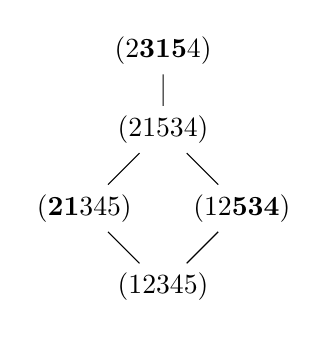
\begin{tikzpicture}[scale=1]
      \node (zero) at (0,-1) {$(12345)$};
      \node (l) at (-1,0) {$({\bf21}345)$};
      \node (r) at (1,0) {$(12{\bf534})$};
      \node (b) at (0,1) {$(21534)$};
      \node (one) at (0,2) {$(2{\bf315}4)$};
      \draw (zero) -- (l) -- (b) -- (one);
      \draw (zero) -- (r) -- (b);
    \end{tikzpicture} 
  \end{tabular}

  Starting from the man-optimal match, the rotations
  $\rho_1=[(1,2),(2,1)]$ and $\rho_2=[(3,3),(4,4),(5,5)]$
  are exposed (this is easily seen
  from the border separated rankings).
  Moreover, once both these rotations have been applied, rotation
  $\rho_3=[(2,1),(4,3),(3,5)]$ is exposed, and eliminating $\rho_3$ gets us to
  the woman-optimal outcome.

  Suppose you flip 1 and 2 first, then woman 2 rejects man 1.
  This leads to a terminal
  phase but also finds rotation $\rho_2$.
  One the other hand, woman 1 rejecting man 2 would start to find $\rho_3$, then
  find $\rho_2$, then complete $\rho_3$.

  \begin{algorithm}
    \caption{MOSM to WOSM Conversion Algorithm}\label{algMosmToWosm}
  \begin{algorithmic}[1]
    \State Let $\mu$ be the man-optimal stable matching
    \State For each man $m$, let $R(m)$ be the set of women who rejected $m$
    during the run of $MPDA$.
    \State Let $S$ be the set of unmatched women in $\mu$
    % \State\Comment $S$ will be those women who have upgraded to their optimal stable match
    \State Set $pred^1_m = \emptyset$ for each man $m$
      \Comment Store the most recent rotation moving $m$
    \State Label each entry of each woman's preference list with $\emptyset$
      \Comment Store the rotation moving $w$ \emph{above} certain men
    \While { $S \ne \W$ }
      \State Store $\tilde\mu \leftarrow \mu$
      \Comment $\tilde\mu$ stores the most recent \emph{stable} match encountered
      \State Pick any $\hat w\in \W\setminus S$
      \State Let $m = \mu(\hat w)$; let $V = [ (m, \hat w) ]$
      \State Set $\mu(\hat w) = \emptyset$ and add $\hat w$ to $R(m)$
        \Comment $\hat w$ rejects $m$

      % \While { $m \ne \emptyset$ }
      \While { $V \ne [\ ]$ }
        \State Let $pred_{m}^2 = \emptyset$
          \Comment Keep track of predecessor rotations
        \State Let $w$ be $m$'s most preferred woman not in $R(m)$

        \While { $\tilde\mu(w) >_w m$ }
          \Comment while $w$ has received a better stable match
          \State Add $w$ to $R(m)$
          \Comment $w$ rejects $m$
          \State If $w$ labeled $m$ with $\rho$, add $\rho$ to $pred_m^2$
          \State \Comment If rotation $\rho$ moved 
            $w$ above $m$, then $\rho$ must precede the current rotation
          \State Update $w$ to $m$'s top woman not in $R(m)$ (or set $w$ to $\emptyset$)
        \EndWhile

        % \State \Comment If $|\M|<|\W|$, then $m$ has had
        %   his proposal accepted by \emph{some} woman $w$
        \State ( So now $m >_w \tilde\mu(w)$ (if $w\ne \emptyset$) )
        \If { $w=\emptyset$ or $w\in S$ }
        \label{lineFirstDeciciveCase}
          \Comment No stable matching exists rotating partners in $V$
          \State Restore $\mu \leftarrow \tilde\mu$
          \State Add all women in $V$ to $S$; Set $V = [\ ]$
          % \State Set $m = \emptyset$

        \ElsIf {$w$ appears in $V$}
          \Comment New rotation found
          \If { $w \ne \hat w$ }
            % \State Set $m_{float} \leftarrow \mu(w) $
            \State Swap $\mu(w) \leftrightarrow m$
            \Comment Subtlety: $w$ does not reject $m$ yet
          \EndIf
          \State \Call{BuildNewRotation}{$w$}

        \ElsIf {$w\notin V$, $w\notin S$} 
          \Comment Continue building rejection chain $V$
          \State Swap $\mu(w) \leftrightarrow m$; Add $w$ to $R(m)$
            \Comment $w$ rejects $\mu(w)$
          \State Append $(m,w)$ to the end of $V$
        \EndIf
        % \State Set $\nu(w) \leftarrow \nu(w)+1$ and $t \leftarrow t+1$

      \EndWhile
    \EndWhile

    \
    \Function{BuildNewRotation}{$w$}
      \State Suppose $V = [(m_1,w_1), (m_2,w_2), \ldots,
        (m_k,w_k)]$ with $w = w_\ell$ for some $\ell \le k$
      \State Update $\tilde\mu(w_i) = \mu(w_i)$ for $i=\ell,\ell+1,\ldots, J$
      \State Remove $\rho^* = [(m_\ell,w_\ell),\ldots,(m_k,w_k)]$ from $V$
      \State Add rotation $\rho^*$ with predecessors
        $\bigcup_{i=\ell}^k pred_{m_i}^1\cup pred_{m_i}^2 $
        to the rotation poset
      \State For each $i=\ell,\ldots,k$, set $pred_{m_i}^1 = \rho^*$
      \State For each $i=\ell,\ldots,k$, and for each man $m$ between 
      $m_i$ and $m_{i-1}$ (or $m_k$ if $i=\ell$) on $w_i$'s list:
      \State \qquad $w$ labels $m$ with $\rho^*$
    \EndFunction
  \end{algorithmic}
  \end{algorithm}

  The algorithm starts from the man-optimal stable outcome (MOSM)
  by running differed acceptance.
  Then it triggers a series of ``divorces'', i.e. it breaks a marriage
  $(m,\hat w)$ and ``continues running differed acceptance''.
  This involves $m$ again proposing down his list until accepted by some woman
  who prefers $m$ to her current best known stable match.
  This ``rejection chain'' can involve cycles, where a woman accepts a proposal
  for the second time. Ignoring cycles for now, the chain can end in one of two
  ways: a ``terminal phase'' in which an element of $\overline\W$
  (the set of women unmatched in the MOSM)
  receives a match, or an ``improvement phase'' in which $\hat w$ receives a
  better stable match.
  A terminal phase clearly cannot constitute a stable match, by the rural
  hospital theorem (claim~\ref{claimRuralDoctors}).
  On the other hand, \cite{AshlagiUnbalancedCompetition17} shows that any
  improvement phase yields a new stable outcome.

  Some notes:
  \begin{itemize}
    % \item When we reach line~\ref{lineFirstDeciciveCase}, we have either
    %   $m >_w \mu(w)$ or $m >_w \tilde\mu(w)$ ((This comment isn't quite necessary,
    %   the next line explain why we actually hit all the cases in the big if else))
    \item The most recent stable match $\tilde\mu$ is stored, while the
      ``partial match'' $\mu$ may not correspond to any stable match.
    \item When $w\in V$, we compare $m$ against $w$'s match in $\tilde\mu$, not in
      $\mu$. This is because we want to make the smallest changes possible that
      result in new stable outcomes, and $w$ will still make an improvement from
      the old stable outcome by accepting this $m$.
    \item If a cycle occurs during a rejection chain, that cycle is immediately 
      ``recorded'' in $\tilde\mu$. This is because this is equivalent to picking
      $\hat w$ to be any woman in the simple cycle, and (similar to differed
      acceptance) the execution of this algorithm is independent of the order in
      which women are picked.
    \item We actually don't need to wait until the rejection chain hits
      $\overline\W$. Instead, we let $S$ denote the set of women for whom we
      know that a phase starting with $\hat w\in S$ will be terminal. If at any
      point a woman in $S$ then accepts the proposal, we know that the phase we
      are currently in will be terminal as well.
  \end{itemize}

  Formally, \cite{AshlagiUnbalancedCompetition17} proves that the following
  all hold during the run of algorithm~\ref{algMosmToWosm}:
  \begin{itemize}
    \item $\tilde\mu$ is always a stable matching.
    \item When a phase is terminal, $\hat w$ is currently matched in $\tilde\mu$
      to her optimal stable partner. Because we eliminate cycles, any other
      woman in $V$ would also cause a terminal phase if she was chosen as 
      $\hat w$. Thus, $S$ always consists of women who have reached their
      optimal stable match.
    \item Every woman is at some point in
      time matched to every stable partner she has, in order from her least
      preferred to her most preferred.
    \item Algorithm~\ref{algMosmToWosm} terminates with $\tilde\mu$ being the
      woman-optimal stable outcome.
  \end{itemize}


\section{Balanced Random Markets}

  For a man $m$ and woman $w$ in some preference set $P$,
  define $R_m(w) := |\{w' : w' \succeq_m w\}|$,
  i.e. the number of women preferred at least as much as $w$,
  i.e. the index of $w$ on $m$'s ordered preference list.
  We will say that $m$ ranks $w$ better than $w'$ when $R_m(w) < R_m(w')$.
  Given a matching $\mu$ stable under preferences $P$,
  define 
  \[ R_{men}(\mu) := \frac{1}{|\M\setminus\overline\M|}
    \sum_{m\in \M\setminus\overline\M} R_m(\mu(m))
  \]
  That is, $R_{men}(\mu)$ is the average over matched men of the men's rank of
  their wives. Define $R_w(m)$ and $R_{women}(\mu)$ analogously.

  A random matching market is defined by a set of randomly draw preferences
  $P = P_{n,m}$ with $n$ men and $m$ women,
  where each of the $n$ men with uniformly random rankings over the $m$ women,
  and $m$ women with uniformly random rankings over the $n$ men.
  Given a set of preferences $P$, let $MOSM(P)$ denote the man-optimal stable
  outcome, i.e. the result of running MPDA (men-proposing differed acceptance).
  Likewise, let $WOSM(P)$ denote the woman-optimal stable
  outcome, i.e. the result of running women-proposing differed acceptance.

  The crucial observations to dealing with MPDA are the following:
  \begin{itemize}
    \item The sum of the ranks that the men have for their wives
      in the MOSM is exactly the number of proposals made during MPDA.
    \item When $n\le m$, MPDA terminates as soon as $n$ distinct women are
      proposed to. Thus, the sum of ranks of the men is essentially a
      \emph{coupon collector} random variable, with expectation $O(\log n)$.
  \end{itemize}

  \begin{proposition}
    Let $P$ be a random matching market with $n$ men and $n+k$ women for $k\ge 0$.
    Then $\E{R_{men}(MOSM(P))}
    = O(\left(\frac{n+k} n\right)\log\left(\frac{n+k}{k}\right))$.
    % and $\E{R_{women}(MOSM(P))} = \Omega(n/\log n)$.
  \end{proposition}
  \begin{proof}
    Consider running men-proposing differed acceptance on $M$.
    At the steps requiring some unmatched man to be selected,
    select one uniformly at random.
    Let $Y$ denote the random variable giving the total number of proposals made
    by men to women.
    By the so-called ``principle of differed decisions'', running this algorithm
    on a random matching market is equivalent to running the following
    randomized algorithm:
    women's preferences are taken as input, but men's are not, and
    whenever a man is ready to propose to a woman, simply select a woman he hasn't
    yet proposed to uniformly at random.

    Let $Z$ denote a ``coupon collector'' random variable defined by the
    following random process: at each step, a uniformly random number in $[n+k]$
    is drawn, and $Z$ returns the number of steps needed for $n$ distinct
    numbers to be draw.
    Note that $Z$ statistically dominates $Y$, because every time a man proposes
    to a woman, he is at least as likely to propose to an unmatched woman as the
    coupon collect step is to select an unselected outcome.

    Now, we have $Z = \sum_{i=1}^n Z_i$, where $Z_i$ is the number of steps
    needed before the $i$th distinct number is draw.
    Observe that $Z_i$ is a geometric random variable with success probability
    $\frac{n+k-i} {n+k}$. Thus:
    \begin{align*}
      \E{Y} & \le \E{Z} \\
        & = \sum_{i=1}^n \E{Z_i} \\
        & = \sum_{i=1}^n \frac{n+k}{n+k-i} \\
        & = (n+k) \sum_{i=k}^{n+k} \frac{1}{i} \\
        & = (n+k)[H_{n+k} - H_k]  \\
        & = \Theta\left( (n+k)[\log(n+k) - \log(k)] \right)  \\
    \end{align*}
    Which gives exactly the desired bound on 
    $\E{R_{men}(MOSM(P))} = \E{Y / n}$.
  \end{proof}

  We can use the above claim to get an informal handle on the expectation
  of $R_{women}(MOSM(P))$ as well.
  In expectation, $O\left((n+k)\log\left(\frac{n+k}{k}\right)\right)$
  proposals are made, so any
  fixed woman $w$ receives an average of
  $O\left(\log\left(\frac{n+k}{k}\right)\right)$ proposals.
  The rank of the men proposing to $w$ is essentially uniformly distributed 
  on $[n]$. The minimum of $h$ uniformly distributed random variables with
  expectation $x$ has expectation $x/h$.
  Thus, the best-ranked man proposing to $w$ has rank
  $\Omega\left(n / \log\left(\frac{n+k}{k}\right) \right)$ on average.

  The previous paragraph can be made formal. A sequence of classical works 
  (in order, \cite{WilsonAnalysisStable72}, \cite{KnuthStableCombinatorial97},
  \cite{PittelAverageStable89}, \cite{PittelLikelyStable92}) got
  quite a good handle on the asymptotic behavior of balanced matching markets.
  Performing a full analysis can get quite complicated, especially when counting
  the \emph{number} of distinct stable matchings\footnote{ 
    This is likely one reason that 
    \cite{AshlagiUnbalancedCompetition17} uses different statistics to measure the
    size of the core, namely, the fraction of agents with multiple distinct
    partners. For many applications, such as the strategic implication of the
    size of the core, this is the more important statistic anyway.
  }.

  % In ((PITEL)), the author gives a much more detailed analysis in order to prove
  % an upper bound on the expected total number of distinct stable matchings.

\section{Unbalanced Random Markets: One Exposition}

  With a little effort, you can extend coupon-collector type arguments to
  get results in the unbalanced case.
  This next claim is adapted from \cite{ImmorlicaHonestyStability05}:
  \begin{claim}
    Consider some matching market $P$ (i.e. a set of preferences
    for men and women) and fix a woman $w^*$ who is matched under any some
    stable matching for $P$.
    Construct preference sets $P_n, P_{n-1}, \ldots, P_1$
    where in $P_i$ we have $w^*$ ``truncate her list'' after place $i$,
    that is, $w^*$ reports her top $i$ choices and deems all other matches
    unacceptable. Let $m_i$ denote the match of $w^*$
    under $MPDA(P_i)$ (or write $m_i = \emptyset$ if $w^*$ is unmatched)
    and let $L = (m_n, m_{n-1}, \ldots, m_1)$.

    We have the following:
    \begin{enumerate}
      \item For each $i$, $\mu_i$ is a stable matching for $P_i$
        with $\mu_i(w^*)\ne \emptyset$
        if and only if $\mu_i$ is a stable matching for $P$.
        % then $\mu_i$ is a stable matching for $P$ if and only if
        % $\mu_i(w^*) \ne \emptyset$.
      \item $L$ is a list containing all the stable matches of $w$,
        possibly with repetition and possibly terminating in a string of
        $\emptyset$s (which do not represent stable matches).
      \item $L$ is ranked from worst to best according to $\prec_w$.
    \end{enumerate}
  \end{claim}
  \begin{proof}
    (1, $\Rightarrow$) If $\mu_i(w^*) = \emptyset$, then we immediately know that
    $\mu_i$ is not stable for $P$, by the rural hospital theorem
    (claim~\ref{claimRuralDoctors} suffices).
    Also, if $\mu_i$ is not stable for $P_i$, then any blocking pair in $P_i$ 
    will also be a blocking pair in $\mu_i$, so $\mu_i$ will not be stable for $P$.

    (1, $\Leftarrow$) Suppose $w^*$ is matched in $\mu_i$,
    and suppose for contradiction that $(m,w)$ is a blocking pair for $\mu_i$
    under $P$. All agents have identical preferences in $P$ and $P_i$ except for
    $w^*$, so we must have $w = w^*$. But because $w^*$ is matched under
    $P_i$, we know $m \succ_{w^*} \mu_i(w^*)$ if and only if
    $m \succ_{w^*}^{(i)} \mu_i(w^*)$ (where $\succ_{w^*}^{(i)}$ denotes $w^*$'s
    preferences in $P_i$). Thus, $(m,w)$ is also blocking for $\mu_i$
    under $P_i$, a contradiction.

    (2, 3) As in the case of full-length preference lists, $MPDA(P_i)$
    will return a stable matching for $P_i$, and it will assign $w^*$ to the
    worst stable partner $w^*$ has under preferences $P_i$, provided one exists.
    By part 1, the stable partners of $w^*$ under $P_i$ are exactly the stable
    partners of $w^*$ under $P$ which are ranked better than place $i$.

    Now, induct on $j$, with the inductive hypothesis being that
    $(m_n, m_{n-1}, \ldots, m_{j})$ contains all stable partners ranked above
    $j$ by woman $w^*$ (in order according to $\prec_{w^*}$).
    The base case is simply the fact that $m_n$ is the worst stable partner of
    $w^*$ (claim~\ref{claimWomenWorstStable}).
    Now, for the inductive step, we have two cases.
    If $m_j$ is still on the preference list of $w^*$ in $P_{j+1}$, then $\mu_j$
    will still be a stable match under preferences $P_{j+1}$. Again by
    claim~\ref{claimWomenWorstStable}, woman $w^*$ will still be matched to
    $m_j$ under preferences $P_{j+1}$.
    On the other hand, if $m_j$ is no longer acceptable to $w^*$ in $P_{j+1}$,
    then $m_{j+1}$ will be the stable partner of $w^*$ which is worst-ranked
    according to $\prec_{w^*}$ (or $\emptyset$ if $w^*$ has already reached her
    best stable match) by the same logic.
    This finishes the proof of the inductive step and of claims 2 and 3.

    % Without loss of generality, suppose $w$ is matched under any
    % stable matching for $P$ (if $w$ is unmatched in $MPDA(P)$,
    % then $m_i=\emptyset$ for each $i$).
    % Let $\mu_i$ be a stable matching for restricted preferences $P_i$.
    % We claim that $\mu_i$ is stable under $P$ if and only if
    % $w$ is matched in $\mu_i$.
    % If $w$ is unmatched, then $\mu_i$ cannot be stable for $P$ by
    % claim~\ref{claimRuralDoctors}.
    % So suppose $w$ is matched in $\mu_i$.

    % First, we show that if $m_i\ne \emptyset$, i.e. $w$ is matched by
    % $MPDA(P_i)$, then the match $\mu_i$ returned by $MPDA(P_i)$ is stable
    % for the original preference set $P$.
    % Indeed, suppose that no pair $(m',w')$, not matched in $\mu_i$,
    % are non-blocking for $P_i$. If $w\ne w'$, then $(m',w')$ cannot be blocking
    % for $P$. So consider $w' = w$. If $w \succ_{m'} \mu_i(m')$,
    % then $m'$ proposed to $w$ during $MPDA(P_i)$.
    % Observe that $w$ only accepts matches above a certain threshold,
    % and once $w$ is matched, her rank of her partner only increases.
    % Thus, as long as $w$ eventually received a match, $\mu_i(w) \succ_w m'$
    % (note that this will not be true if $w$ is unmatched in the end).

    % Now, by the above paragraph, when $m_i\ne\emptyset$, $MPDA(P_i)$
    % returns a stable match of $w$ ranked higher than place $i$.
    % By claim~\ref{claimWomenWorstStable}, it returns the \emph{worst}
    % such stable partner.

    % Now, we induct on $i$ to show that $L$ contains all stable matches of $w$ in
    % order according to $\prec_w$.
    % The base case, that $m_n = \worst(w)$, is just
    % claim~\ref{claimWomenWorstStable}.
    % because $w$ only accepts matches above some threshold any match, she will only upgrade.
  \end{proof}

  We get this immediate corollary:
  \begin{corollary}\label{corTruncateOptimal}
    Suppose that when a woman $w^*$ truncates her preference list after place
    $i$, she is unmatched by MPDA.
    Then $w^*$ has no stable parters ranked better than $i$.
  \end{corollary}

  We are now ready to prove the main result of this section.
  We focus on the case of $n$ men and $n+1$ women, for simplicity.
  I'm still working on making this bit fully formal.

  \begin{claim}
    Consider a random matching market with $n$ men and $n+1$ women.
    Fix some woman $w^*$.
    With probability approaching $1$ as $n\to\infty$, % $1 - O((\log n)^{-2})$,
    $w^*$ has no stable partners ranked better than $\Omega(n/\log n)$.
    % fewer than $\Theta(n\log n)$ proposals are made by the men
    % before $MPDA$ terminates. 
    % Moreover, fewer than $\log n$ proposals are made to $w^*$.
  \end{claim}
  \begin{proof}[(Proof Sketch)]
    Suppose $w^*$ truncates her preference list at place $c n / \log n$ for some
    constant $c$. Denote this preference list by $P^*$.
    By corollary~\ref{corTruncateOptimal}, $w^*$ has a stable partner ranked
    better than $c n/\log n$ if and only if $w^*$ is matched under $MPDA(P^*)$.
    This occurs if and only if $w^*$ receives a proposal from a man ranked
    better than $c n/\log n$.
    But when a man proposes to $w^*$, his rank by $w^*$ is uniformly distributed
    (over those ranks $w^*$ has not yet seen in the algorithm).
    To proceed, we upper bound the number of proposals that $w^*$ likely
    receives, and thus the probability that she gets a proposal ranked higher
    than $c n/\log n$. 

    Let $Y$ denote the random variable giving the number of proposals $w^*$ sees
    during the run of $MPDA(P^*)$.
    First, note that $MPDA(P^*)$ will certainly terminate if all women other
    than $w^*$ have been proposed to.
    Thus, $Y$ is statistically dominated by the following variation on a coupon
    collector random variable:
    define a process which at each step selects a number uniformly at random
    from $[n+1]$. The process terminates when each number in $[n]$ has been
    selected, and $Z$ outputs the number of times $n+1$ was selected.
    We have $Y$ statistically dominated by $Z$.

    Now, because the standard coupon collector random variable has expectation
    $O(n\log n)$, this modified coupon collector should have expectation
    $O(\log n)$. Thus, in expectation, the best ranked man who proposes to
    $w^*$ has rank $\Omega( n /\log n )$.

    % We again divide $Z$ into ``stages'' $Z = \sum_{i=1}^n Z_i$, where $Z_i$
    % gives the number of times $n+1$ is selected between the $i-1$th and $i$th
    % distinct number from $[n]$ being selected.
    % Let $N_i$ denote the number of draws between the $i-1$th and $i$th distinct
    % draw from $[n]$.

    % Let $Y$ denote the number of time $w^*$ is proposed to.
    % $MPDA$ will terminate as soon as $n$ distinct women are proposed to.
    % This is still dominated by a coupon collector random variable.

    % In expectation, $\Theta(\log n)$ of those proposals go to $w^*$.
  \end{proof}



\section{\cite{AshlagiUnbalancedCompetition17} and MOSM to WOSM Conversion}

  For this section, we always assume $|\M| = |\W| + k$ for $k > 0$.
  The main algorithm used in the analysis of
  \cite{AshlagiUnbalancedCompetition17} is given here in
  Algorithm~\ref{algMosmToWosm}.
  To understand this algorithm fully, I've actually implemented it
  at \url{https://github.com/ClathomasPrime/CompetitiveStableMatching}.
  It is presented here in a more ``imperative programming'' style than that
  given in \cite{AshlagiUnbalancedCompetition17}

  Finally, \cite{AshlagiUnbalancedCompetition17} shows that the core of an
  unbalanced market is probably small by showing that
  algorithm~\ref{algMosmToWosm} probably terminates quickly.
  Thus, there cannot be a big difference between the man-optimal and the woman
  optimal stable matches: most agents have unique stable partners, and the
  average ranks for agent's partners is about the same in all matchings.
  This is a long, involved probabilistic argument, but is terribly difficult to
  carry out. The result is:

  \begin{theorem}[\cite{AshlagiUnbalancedCompetition17}, Appendix B]
    Consider any sequence of random matching markets with $n$ men and $n+k$ women
    (for any $k = k(n) \ge 1$).
    For any $\epsilon>0$, with probability that approaches $1$ as $n\to\infty$,
    each of the following events hold:
    \begin{enumerate}
      \item Define $ s_k(n) := \left(\frac{n+k} n\right) 
        \log\left(\frac{n+k} k\right)$.
        Then for every stable matching $\mu$,
        \begin{align*}
          R_{men}(\mu) \le (1+\epsilon)s_k(n) &&
          R_{women}(\mu) \ge \frac n {1 + (1+\epsilon)s_k(n)}
        \end{align*}
      \item Less than a $1/\sqrt{\log n}$ fraction of the men and women have
        multiple stable partners. In particular, this fraction approaches $0$ as
        $n\to\infty$.
        Moreover, the total number of stable partners
        is at most $n + n/\sqrt{\log n}$.
      \item There is little difference in ranking between the MOSM and the WOSM:
        \begin{align*}
          \frac{R_{men}(WOSM)}{R_{men}(MOSM))} \le 1+\epsilon &&
          \frac{R_{women}(WOSM)}{R_{women}(MOSM))} \ge 1-\epsilon
        \end{align*}
    \end{enumerate}
  \end{theorem}

  Comparing this to the results from section 3, we see that when imbalance is
  present, men \emph{almost always} do as well in \emph{any} stable matching as
  they do in the man-optimal stable matching.
  Two special cases are worth pointing out:

  \begin{corollary}[2.2 in \cite{AshlagiUnbalancedCompetition17}]
    Suppse $k(n) = 1$ for each $n$.
    Then for every $\epsilon>0$, with probability approaching $1$ as
    $n\to\infty$, we have
    \begin{align*}
      R_{men}(\mu) \le (1+\epsilon)\log n &&
      R_{women}(\mu) \ge (1-\epsilon)\frac n {\log n}
    \end{align*}
    for every stable matching $\mu$.
  \end{corollary}

  \begin{corollary}[2.3 in \cite{AshlagiUnbalancedCompetition17}]
    Suppse there exists a $\lambda >0$ with $k(n) = \lambda n$ for each $n$.
    Let $\kappa = (1 + \lambda)\log(1 + 1/\lambda)$.
    Then for every $\epsilon>0$, with probability approaching $1$ as
    $n\to\infty$, we have
    \begin{align*}
      R_{men}(\mu) \le (1+\epsilon)\kappa &&
      R_{women}(\mu) \ge (1-\epsilon)\frac n {1 + \kappa}
    \end{align*}
    for every stable matching $\mu$.
  \end{corollary}

  In a follow-up paper \cite{PittelLikelyStableUnbalanced19}, many of these
  results are shown to be sharp, and the analysis is extended to count the
  average number of stable matchings in an unbalanced market.
  Interestingly, \cite{PittelLikelyStableUnbalanced19} is not able to improve
  the rate at which the fraction of agents with multiple stable partners tends
  to zero as $n\to\infty$, even though the arguments in section 4 seem to
  suggest that this fraction might be about $1/\log n$.

  % \subsection{Relation to the rotation poset}
  It's worth noting that algorithm~\ref{algMosmToWosm} is almost identical to the
  algorithm \emph{minimal-differences} described
  in~\cite{GusfieldStableStructureAlgs89} (a book which fully fleshes out
  ideas initiated in~\cite{IrvingCountingStable86}).
  The purpose of algorithm \emph{minimal-differences} is to traverse the
  matching lattice in a maximal chain from the MOSM to the WOSM, and along the
  way identify ``the rotation poset'' (i.e. the poset for which the matching
  lattice is the collection of downwards-closed sets of the poset, which is
  guaranteed to exist by Birkhoff's representation theorem).
  The only difference is that algorithm~\ref{algMosmToWosm} does not explicitly
  identify the ``rotations'' (i.e. simple improvement cycles).
  \cite{AshlagiUnbalancedCompetition17}'s careful analysis of this algorithm
  for unbalanced random markets essentially says that the rotation poset, and
  consequentially the stable matching lattice, is typically small (in a few very
  precise ways).

    % It's not clear if the authors of \cite{AshlagiUnbalancedCompetition17} realize this.


  % \begin{proof}
  %   Induct on the length of $V$ and the size of $S$.
  %   If $|V| = 1$, then 
  %   UUGH well this still gets a bit messy. Probably best to use known proofs.
  %   I think it would work IF you show a converse of the ``lattice neighbors
  %   covering'' thing: all guys hasse-adjacent in the lattice differ by an
  %   improvement cycle.
  % \end{proof}

\bibliography{MechDesign}{}
\bibliographystyle{alpha}

\appendix

\section{The Error in \cite{GusfieldStableStructureAlgs89}}

The algorithm of \cite{GusfieldStableStructureAlgs89} correctly identifies all
of the rotations in a stable matching instance. However, there is a slight error
in the construction of the order relations for the rotation poset.
In particular, once the rotations are found (via an algorithm essentially
equivalent to our algorithm~\ref{algMosmToWosm}), they propose the following:
\begin{algorithm}
  \caption{Construct rotation ordering}\label{algRotationOrderGI}
\begin{algorithmic}[1]
  \For {Each rotation $\rho$ and pair $(m_i,w_i)\in \rho$}
    \State Label $w_i$ in $m_i$'s preference list with a type 1 $\rho$ label
    \For {Each $m$ strictly between $m_i$ and $m_{i-1}$ on $w_i$'s list}
      % \Comment $w_i$ upgrades $m_i$ to $m_{i-1}$
      \State Label $w_i$ in $m$'s preference list with a type 2 $\rho$ label
    \EndFor
  \EndFor
  \For {Each man $m$}
    \State Set $\rho^* = \emptyset$
    \For {Each woman $w$ on $m$'s preference list, in order}
      \If {$w$ has a type 1 label of $\rho$}
        \If { $\rho^* \ne \emptyset$ } 
          Add $\rho^*$ as a predecessor of $\rho$
        \EndIf
        \State Set $\rho^* = \rho$
      \EndIf
      \If { $w$ has a type 2 label of $\rho$}
        \If {$\rho^*\ne \emptyset$}
          Add $\rho$ as a predecessor of $\rho^*$
        \EndIf
      \EndIf
    \EndFor
  \EndFor
\end{algorithmic}
\end{algorithm}

The idea behind this algorithm is very sound:
Suppose the labeled women on $m$'s preference list consist of
of $m$ has woman $w$ on his preference list,
and rotation $\rho$ moves $w$ from below to above $m$
on her own preference list.


\end{document}
